\documentclass{hw-template}

\title{NE523 Homework 2}
\author{Kyle Hansen}
\date{18 February 2026}

\usepackage{cancel}

\renewcommand{\defeq}{\stackrel{\text{def}}{=}}




\begin{document}

\maketitle{}

\section{Fluxes \& Currents}

Angular flux $\psi({\hat{\Omega}})$ is the intensity of neutrons in the direction $\hat{\Omega}$. In this case, since the intensity is $I$ when in direction $\hat{i}$ (the unit vector in the $x$-direction), and zero otherwise. So,

\begin{equation}
    \psi(\hat{\Omega}) = I\delta(\hat{i}\cdot \hat{\Omega} - 1),
\end{equation}

since $\hat{i}\cdot \hat{\Omega}=1$ when $\hat{\Omega} = \hat{i}$. Then, using this angular flux,

\begin{equation}
    \varphi = \int\limits_{4\pi}d\Omega \; I\delta(\hat{i}\cdot \hat{\Omega} - 1) = I.
\end{equation}

The current vector is

\begin{equation}
    \vec{J} = \int\limits_{4\pi}d\Omega\; \hat{\Omega}\psi  = \hat{i}I,
\end{equation}

and the partial currents are 

\begin{equation}
    J_x^+ = \int\limits_{\hat{\Omega}\cdot \hat{i}>0}d\Omega\; \hat{i}\cdot\hat{\Omega}\psi = I
\end{equation}

\begin{equation}
    J_x^- = \int\limits_{\hat{\Omega}\cdot \hat{i}<0}d\Omega\; \hat{i}\cdot\hat{\Omega}\psi = 0
\end{equation}

\section{Slab Geometry Transport Solution}

The transport equation for a purely absorbing medium with isotropic source is

\begin{equation}
    \hat{\Omega}\cdot \nabla \psi(\vec{r}, \hat{\Omega}, E) + \sigma_t\psi = \frac{1}{4\pi}q(E).
\end{equation}

Then, since in slab geometry $\frac{d\psi}{dy} = \frac{d\psi}{dz} = 0$, this becomes

\begin{equation}
    \mu \frac{d}{dx}\psi(x, \hat{\Omega}, E) + \sigma_t \psi = \frac{1}{4\pi}q(E).
\end{equation}

Since this is a seperable ODE, the solution can be found by rearranging and integrating both sides:


\begin{align}
    -\mu \frac{d\psi}{dx} &= \sigma_t \psi(x, \hat{\Omega}, E) - \frac{1}{4\pi}q(E) \\
    \frac{1}{ \sigma_t \psi(x, \hat{\Omega}, E)  - \frac{1}{4\pi}q(E)} d\mu &= \frac{-1}{\mu}dx\\
    \int \frac{1}{ \sigma_t \psi(x, \hat{\Omega}, E)  - \frac{1}{4\pi}q(E)} d\mu &=-\int \frac{1}{\mu}dx\\
    \frac{\ln\left(\sigma_t \psi(x, \hat{\Omega}, E)  - \frac{1}{4\pi}q(E)\right)}{\sigma_t} &= -\frac{x}{\mu} + c_0\\
    \sigma_t \psi (x, \hat{\Omega}, E) - \frac{1}{4\pi}q(E) &= c_1 e^{-\frac{\sigma_t}{\mu}x}\\
    \sigma_t \psi(x, \hat{\Omega}, E)   &= c_1 e^{-\frac{\sigma_t}{\mu}x} + \frac{1}{4\pi}q(E)\\
    \psi(x, \hat{\Omega}, E)   &= c_2 e^{-\frac{\sigma_t}{\mu}x} + \frac{1}{4\pi\sigma_t }q(E).
\end{align}

The boundary conditions are different for different values of $\mu$; for $\mu>0$, the constant $c_2=0$ since $\psi$ must be finite for the left half of the domain. For $\mu<0$, the incoming flux boundary condition $\psi(0, \mu<0) = 0$ can be used, and the constant becomes $c_2 = -\frac{1}{4\pi \sigma_t} q(E)$. Then in the slab, the flux is

\begin{equation}
    \psi(x, E)   = \begin{cases}
    \frac{1}{4\pi\sigma_t }q(E), & \mu>0\\
    \frac{1}{4\pi\sigma_t }q(E) \left(1 - e^{\frac{\sigma_t}{\mu}x} \right), & \mu<0
    \end{cases} , \quad -\infty \leq x < 0.
\end{equation}

At the interface $x=0$, since there is no incoming flux from the vacuum, 

\begin{equation}
    \psi(0, \Omega, E) = \begin{cases}
        \frac{1}{4\pi\sigma_t }q(E), & \mu\geq0\\
        0, & \mu < 0\\
    \end{cases}
\end{equation}

and the current vector is

\begin{equation}
    \vec{J}(0, E) = \int\limits_{4\pi}d\Omega \; \hat{\Omega}\psi = \hat{i}\frac{1}{2}q(E)
\end{equation}

\section{Inner Products \& Orthogonality}

For the set of polynomials to be orthonormal on $x \in [-1, 1]$, they must satisfy the condition that $\ip{P_i}{P_j} = \int_{-1}^{1}P_iP_j dx = \delta_{i, j}$:

\begin{equation}
    \begin{aligned}
    \ip{P_0}{P_0} &= \int\limits_{-1}^{1} \frac{1}{\sqrt{2}}\cdot \frac{1}{\sqrt{2}} dx\\
    &=\frac{1}{2} \int\limits_{-1}^{1}  dx\\
   \ip{P_0}{P_0} &= \boxed{1}
\end{aligned}
\end{equation}
\hrule
\begin{equation}
    \begin{aligned}
        \ip{P_0}{P_1} &= \int\limits_{-1}^{1} \frac{1}{\sqrt{2}}\cdot \frac{\sqrt{3}}{\sqrt{2}}x dx\\
        &=\frac{1}{2} \int\limits_{-1}^{1} x dx\\
        &=\frac{1}{2} \left[\frac{x^2}{2} \right]_{-1}^{1} \\
        &=\frac{1}{2} \left[\frac{1}{2} - \frac{1}{2}\right]\\
        \ip{P_0}{P_1} &= \boxed{0}
    \end{aligned}
\end{equation}
\hrule
\begin{equation}
    \begin{aligned}
        \ip{P_0}{P_2} &= \int\limits_{-1}^{1} \frac{1}{\sqrt{2}}\cdot \frac{\sqrt{5}}{\sqrt{2}} \cdot \frac{1}{2} \left(3x^1 - 1 \right)dx\\
        &= \frac{\sqrt{5}}{4}\int\limits_{-1}^{1}  \left(3x^2 - 1 \right)dx\\
        &= \frac{\sqrt{5}}{4} \left[ x^3 - x \right]_{-1}^{1}\\
        &= \frac{\sqrt{5}}{4} \left[ \left(1-1 \right) - \left(1-1 \right) \right]\\
        \ip{P_0}{P_2} &= \boxed{0}
    \end{aligned}
\end{equation}
\hrule
\begin{equation}
    \begin{aligned}
    \ip{P_1}{P_1} &= \frac{3}{2}\int\limits_{-1}^{1} x^2 dx\\
     &= \frac{3}{2} \left[ \frac{x^3}{3} \right]_{-1}^1\\
    &= \frac{3}{2} \left[ \frac{1}{3} - \frac{-1}{3} \right]_{-1}^1\\
    \ip{P_1}{P_1} &= \boxed{1}
\end{aligned}
\end{equation}
\hrule
\begin{equation}
    \begin{aligned}
    \ip{P_1}{P_2} &= \sqrt{\frac{3}{2}}\sqrt{\frac{5}{2}}\int\limits_{-1}^{1} \frac{1}{2}x  \left(3x^2 - 1 \right)dx\\
    &= \frac{\sqrt{15}}{2}\int\limits_{-1}^{1} \frac{3}{4}x^2 - \frac{1}{2}x \, dx\\
    &= \frac{\sqrt{15}}{2} \left[ \frac{3}{8}x^4 - \frac{1}{4}x^2 \right]_{-1}^{1}\\
    &= \frac{\sqrt{15}}{2} \left[ \left(\frac{3}{8} - \frac{1}{4} \right) - \left( \frac{3}{8} - \frac{1}{4}\right) \right]\\
    \ip{P_1}{P_2} &= \boxed{0}
\end{aligned}
\end{equation}
\hrule
\begin{equation}
    \begin{aligned}
    \ip{P_2}{P_2} &= \frac{5}{2} \int\limits_{-1}^{1} \frac{1}{2^2} \left(3x^2 - 1 \right)^2dx\\
    &= \frac{5}{8} \int\limits_{-1}^{1}  9x^4 - 6x^2 + 1\,dx\\
    &= \frac{5}{8} \left[ \frac{9}{5}x^5 - 2x^3 + x \right]_{-1}^{1}\\
    &= \frac{5}{8} \left[ \left(\frac{9}{5} - 2 + 1 \right) -  \left(\frac{-9}{5} + 2 - 1 \right) \right]\\
    \ip{P_2}{P_2} &= \boxed{1}.
\end{aligned}
\end{equation}

This confirms the condition that $\ip{P_i}{P_j}  = \delta_{i, j}$, so the set of polynomials is orthonormal.

\section{Projection on Orthogonal Basis}

Any quantity (function, vector, etc) can be represented as a linear conbination of orthonormal basis componenents, with coefficients equal to the magnitude of a projection onto those bases. For functions on $x\in[-1, 1]$, using the Legendre polynomials as a basis, this expansion is

\begin{equation}
    f(x) = \sum_l^\infty \frac{\ip{f}{P_l}}{\ip{P_l}{P_l}} P_l.
\end{equation}

since $\ip{P_l}{P_l} = 1$, the coefficients (``moments'') are $f_l = \ip{f}{P_l}; l=0, \dots, \infty$. Assuming that the series $\sum_{l=0}^L f_lP_l$ converges to $f(x)$ (that is, each successive term in the sequence of truncated reconstructions is closer to the true function than the previous term), the function can be approximated using only the first $L+1$ terms.

\subsection{}

The Legendre moments are

\begin{equation}
    f_i = \ip{f(x)}{P_i(x)} = \int\limits_{-1}^{1}.
\end{equation}

Then, for $f(x) = 3x+7$, 

\begin{equation}
    \begin{aligned}
      f_0 &= \int\limits_{-1}^{1} \frac{1}{\sqrt{2}}\left(3x + 7 \right)dx\\
    &= \frac{1}{\sqrt{2}}\left[ \frac{3}{2}x^2 + 7x \right]_{-1}^{1}\\
    &= \frac{1}{\sqrt{2}}\left[ \left(\frac{3}{2} + 7\right) - \left(\frac{3}{2} - 7 \right)  \right]\\
    &= \frac{1}{\sqrt{2}}\left[ 14\right]\\
    &= \frac{14}{\sqrt{2}}\\
    f_0 &= 7\sqrt{2}  
    \end{aligned}
\end{equation}

\begin{equation}
    \begin{aligned}
    f_1 &= \frac{\sqrt{3}}{\sqrt{2}}\int\limits_{-1}^{1} x\left(3x + 7 \right)dx\\
    &=\frac{\sqrt{3}}{\sqrt{2}} \left[ x^3 +  \frac{7}{2}x^2\right]_{-1}^{1}\\
    &=\frac{\sqrt{3}}{\sqrt{2}} \left[ \left(1 +\frac{7}{2} \right) - \left(-1 +\frac{7}{2} \right) \right]\\
    &=\frac{2\sqrt{3}}{\sqrt{2}}\\
    f_1 &= \sqrt{6} 
    \end{aligned}
\end{equation}

\begin{equation}
    \begin{aligned}
        f_2 &= \frac{\sqrt{5}}{\sqrt{2}}\int\limits_{-1}^{1} \frac{1}{2} \left(3x^2 -1 \right)\left(3x + 7 \right)dx\\
        &= \frac{1}{2}\frac{\sqrt{5}}{\sqrt{2}}\int\limits_{-1}^{1} \left( 9x^3 -3x + 21x^2 - 7 \right) dx\\
        &= \frac{1}{2}\frac{\sqrt{5}}{\sqrt{2}} \left[ \frac{9}{4}x^2 - \frac{3}{2}x^2 + 7x^3 - 7x \right]_{-1}^{1}\\
        f_2 &= 0
    \end{aligned}
\end{equation}


Because the original function is a polynomial with degree less than two, the truncated Legendre expansion is equal to the original funciton, as seen in \autoref{fig:parta}.

\begin{figure}
    \centering
    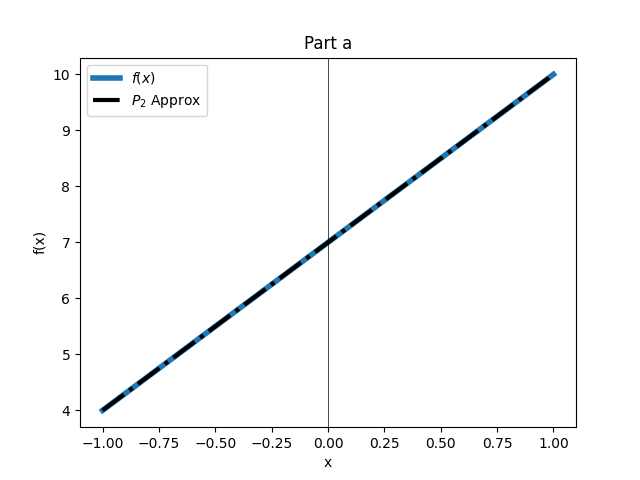
\includegraphics[width=0.65\linewidth]{parta.png}
    \caption{Function and approximation, Part a}\label{fig:parta}
\end{figure}


\subsection{}

For the function $f(x) = e^x$, 

\begin{equation}
    \begin{aligned}
        f_0 &= \frac{1}{\sqrt{2}} \int\limits_{-1}^{1} e^x dx\\
        &= \frac{1}{\sqrt{2}} \left[e^x \right]_{-1}^{1}\\
         f_0 &= \frac{1}{\sqrt{2}} \left[e^1 - e^{-1} \right]\\
    \end{aligned}
\end{equation}

\begin{equation}
    \begin{aligned}
        f_1 &= \sqrt{\frac{3}{2}} \int\limits_{-1}^{1} xe^x dx\\
        &= \sqrt{\frac{3}{2}} \left[\left.xe^x \right\vert_{-1}^{1} - \int\limits_{-1}^{1} e^x dx \right]\\
        &= \sqrt{\frac{3}{2}} \left[ \left(e^1 + e^{-1} \right) - \left(e^1 - e^{-1} \right) \right]\\
        f_1&= \sqrt{6} e^{-1}\\
    \end{aligned}
\end{equation}

\begin{equation}
    \begin{aligned}
        f_2 &= \frac{1}{2}\sqrt{\frac{5}{2}} \int\limits_{-1}^{1}  \left(3x^2 - 1 \right) e^x dx\\
        &= \frac{1}{2}\sqrt{\frac{5}{2}} \left[ \left.  e^x \left(3x^2 - 1 \right)\right\vert_{-1}^{1} - \int\limits_{-1}^{1}6xe^x dx \right]\\
        &= \frac{1}{2}\sqrt{\frac{5}{2}} \left[ \left[  e^x \left(3x^2 - 1 \right) -   6xe^x \right]_{-1}^{1} + \int\limits_{-1}^{1}6e^x dx \right]\\
        &= \frac{1}{2}\sqrt{\frac{5}{2}} \left[ e^x \left( 3x^2 -6x -1 + 6\right)\right]_{-1}^{1}\\
        &= \frac{1}{2}\sqrt{\frac{5}{2}} \left[ e^x \left( 3x^2 -6x +5 \right)\right]_{-1}^{1}\\
        &= \frac{1}{2}\sqrt{\frac{5}{2}} \left[ e^1 \left(3 - 6 + 5 \right) - e^{-1} \left( 3 + 6 + 5\right)\right]\\
        f_2 &= \frac{1}{2}\sqrt{\frac{5}{2}} \left[2e^1 - 14e^{-1}\right]\\
    \end{aligned}
\end{equation}


Though the function is exponential, the truncated Legendre approximation is still close with only three moments used, as seen in \autoref{fig:partb}.

\begin{figure}
    \centering
    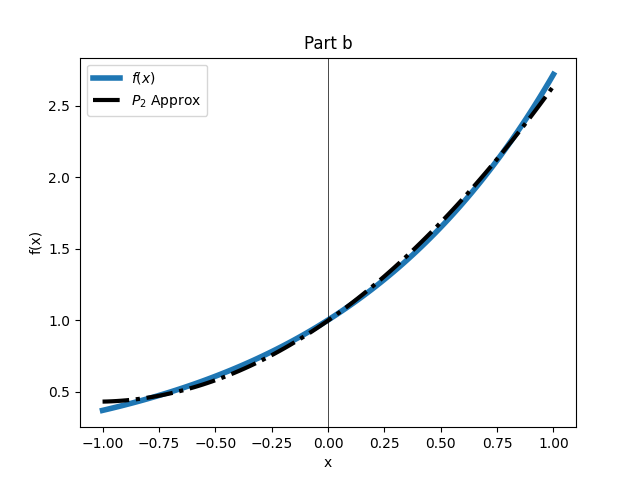
\includegraphics[width=0.65\linewidth]{partb.png}
    \caption{Function and approximation, Part b}\label{fig:partb}
\end{figure}

\subsection{}

For the function $f(x) = e^{5x}$, 


\begin{equation}
    \begin{aligned}
        f_0 &= \frac{1}{\sqrt{2}}\int\limits_{-1}^{1}e^{5x}dx\\
        &= \frac{1}{\sqrt{2}}\left[\frac{1}{5}e^{5x} \right]_{-1}^{1}\\
        f_0&= \frac{1}{5\sqrt{2}}\left[e^5 - e^{-5}\right]\\
    \end{aligned}
\end{equation}

\begin{equation}
    \begin{aligned}
        f_1 &= \sqrt{\frac{3}{2}} \int\limits_{-1}^{1}xe^{5x}dx\\
        &= \sqrt{\frac{3}{2}} \left[  \left.  \frac{1}{5} xe^{5x}\right\vert_{-1}^{1}   - \int\limits_{-1}^{1}\frac{1}{5}e^{5x}dx\right]\\
        &= \sqrt{\frac{3}{2}} \left[ \frac{1}{5}xe^{5x} - \frac{1}{25}e^{5x} \right]_{-1}^{1}\\
        &= \frac{1}{5}\sqrt{\frac{3}{2}} \left[ \left( e^5 - \frac{1}{5}e^{-5}\right) - \left( -e^5 - \frac{1}{5}e^{-5}\right)\right]\\
        f_1&= \frac{1}{25}\sqrt{\frac{3}{2}} \left[ 4 e^5 + 6e^{-5}\right]
    \end{aligned}
\end{equation}

\begin{equation}
    \begin{aligned}
        f_2 &= \frac{1}{2}\sqrt{\frac{5}{2}}  \int\limits_{-1}^{1} e^{5x} \left(3x^2 - 1 \right)dx\\
        &= \frac{1}{2} \sqrt{\frac{5}{2}} \left[\int\limits_{-1}^{1} 3x^2 e^{5x} dx - \int\limits_{-1}^{1} e^{5x} dx \right]\\
        &= \frac{1}{2}\sqrt{\frac{5}{2}}  \left[\left. \frac{3}{5}x^2 e^{5x}\right\vert_{-1}^{1} - \int\limits_{-1}^{1} \frac{6}{5}x e^{5x} dx - \left. \frac{1}{5}e^{5x}\right\vert_{-1}^{1} \right]\\
        &= \frac{1}{2} \sqrt{\frac{5}{2}} \left[ \left(\frac{3}{5}x^2 e^{5x}- \frac{6}{25}xe^{5x} -\frac{1}{5}e^{5x}  \right)_{-1}^1 + \int\limits_{-1}^{1} \frac{6}{25}e^{5x}dx \right]\\
        &= \frac{1}{2}\sqrt{\frac{5}{2}}  \left[ \frac{3}{5}x^2 e^{5x}- \frac{6}{25}xe^{5x} -\frac{1}{5}e^{5x}  + \frac{6}{125}e^{5x} \right]_{-1}^1\\
        &= \frac{1}{2}\sqrt{\frac{5}{2}}  \left[ \left(\frac{75}{125}x^2 -  \frac{30}{125}x +  \frac{19}{125} \right) e^{5x}\right]_{-1}^1\\
        &= \frac{1}{250}\sqrt{\frac{5}{2}}  \left[ \left(75x^2 -  30x +  19 \right) e^{5x}\right]_{-1}^1\\
        &= \frac{1}{250}\sqrt{\frac{5}{2}}  \left[ \left(75-30-19 \right)e^{5} - \left(75+30-19 \right)e^{-5}\right]\\
        f_2 &= \frac{1}{250}\sqrt{\frac{5}{2}}  \left[ 26e^{5} - 86e^{-5}\right]\\
    \end{aligned}
\end{equation}


Because of the rapid growth of $e^{5x}$, this function is poorly approximated with polynomials, as seen in \autoref{fig:partc}.


\begin{figure}
    \centering
    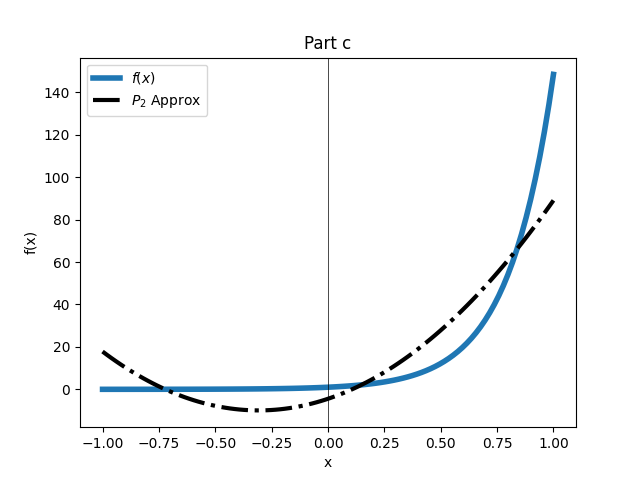
\includegraphics[width=0.65\linewidth]{partc.png}
    \caption{Function and approximation, Part c}\label{fig:partc}
\end{figure}




\end{document}
